% Editable research draft. Compile main.tex with pdfLaTeX + BibTeX.
% Replace author details, confirm dataset rights/citations, and apply the venue template.
\documentclass[11pt,a4paper]{article}
\usepackage[margin=0.85in]{geometry}
\usepackage[T1]{fontenc}
\usepackage[utf8]{inputenc}
\usepackage{lmodern,microtype,amsmath,amssymb,booktabs,graphicx}
\usepackage[numbers,sort&compress]{natbib}
\usepackage{tikz}
\usetikzlibrary{positioning,arrows.meta}
\usepackage{xcolor}
\usepackage[hidelinks]{hyperref}
\usepackage{url}
\setlength{\emergencystretch}{3em}
\title{Context-Aware Toxicity Classification with Hierarchical IndicBERT and Conservative Expert Blending:\\An Exploratory Multisource Evaluation}
\author{Author names and affiliations to be supplied}
\date{}
\begin{document}
\maketitle
\begin{center}\small\textbf{Manuscript draft: author information, data attribution/rights and venue formatting require final review.}\end{center}

\begin{abstract}
Toxicity classification must distinguish the target message from the surrounding conversation while handling inputs with missing or variable-length history. We implement a hierarchical IndicBERT-v2 classifier over genuine ancestor chains and combine its predictions with lexical classifiers. We then compare a validation-selected, script-conditioned blend of existing English and mixed-language experts against its constituent models. The cleaned training and evaluation pool contains 78,232 targets from English personal-attack, Telugu prompt-safety and Tamil code-mixed offensiveness sources. On 11,878 test targets, the adaptive method obtains positive-class F1 of 0.7299, compared with 0.7284 for the mixed ensemble; the paired 95\% interval for the difference includes zero. On 2,282 contextual English targets, removing parents reduces average precision from 0.8754 to 0.8560, with a positive exploratory paired interval, but the corresponding F1 interval includes zero. Reversed and unrelated-parent controls show little separation from genuine context. On a 51-target authored Telugu/Romanized development challenge, adaptive F1 is 0.6222 versus 0.6522 for the mixed ensemble. The contribution is a reproducible integration and empirical analysis of expert specialization and context sensitivity, rather than a new encoder or demonstrated universal improvement.
\end{abstract}

\section{Introduction}
A target reply may be interpreted differently depending on preceding messages. However, a toxic ancestor does not imply that its reply is toxic, and available history is not necessarily informative. Contextual toxicity and context-sensitivity estimation have already been studied~\citep{pavlopoulos2020,xenos2021}. Practical systems must therefore evaluate the incremental value of context instead of assuming it.

This work addresses three questions: (RQ1) how do English-specialized and mixed-language experts differ across source populations; (RQ2) does a restricted script-conditioned combination improve on an existing mixed ensemble; and (RQ3) is any measured advantage from parent history robust to removal and control-context changes? Our task is classification of the current target using observed ancestors, not forecasting a future conversational failure. Consequently, our use of Conversations Gone Awry (CGA) is not directly comparable with its original forecasting benchmark~\citep{zhang2018}.

The contributions are an implemented ancestry-aware pipeline with an explicit target representation; a conservative, validation-selected comparison of lexical/neural expert combinations; and reproducible source-specific, depth-specific and context-control diagnostics. We do not claim priority for contextual toxicity detection, Transformer pooling, LoRA or soft voting. The study is exploratory because base models reused the original validation population, and earlier test analyses informed subsequent project development.

\section{Related Work}
BERT established pretrained bidirectional Transformer representations~\citep{devlin2019}; IndicBERT v2 provides an Indic-language-oriented pretrained model~\citep{doddapaneni2023}. LoRA adapts pretrained weight matrices through low-rank updates~\citep{hu2021}. We reuse these established components and do not propose changes to their pretraining objectives.

CGA studies early signs of conversational breakdown~\citep{zhang2018}. We instead extract labelled target comments and their actual reply ancestry. Work on contextual toxicity examines whether surrounding posts alter classification~\citep{pavlopoulos2020}; context-sensitivity estimation explicitly studies when context should be considered~\citep{xenos2021}. These precedents limit a broad novelty claim for routing between context-sensitive and context-free systems. Our narrower empirical focus is the interaction between lexical/neural expert specialization, script ambiguity and context diagnostics on the project's fixed source populations. This is not an exhaustive systematic literature review or a state-of-the-art comparison.

\section{Data and Preprocessing}
The cleaned pool includes English CGA personal-attack comments, a mapped subset of Cultural-Safety-Telugu~\citep{telugucard}, and Tamil code-mixed offensiveness data from the named DravidianCodeMix distribution~\citep{tamilcard}. As summarized in Table~\ref{tab:data}, the combined pool comprises 78,232 targets across grouped train, validation, and test partitions. Telugu safety prompts are not natural threaded Telugu conversations. The Tamil source is not a Telugu code-mixed benchmark. Source labels have different meanings despite their binary encoding, so per-source results are primary and pooled results are descriptive.

For Tamil, the local adapter maps label 0 to non-offensive, drops label 1 (not-Tamil), and maps labels 2--5 to offensive. The Telugu adapter selects toxicity-related safety categories and excludes unrelated unsafe-request categories; its mapping includes harassment/profanity, hate/identity attacks, violence/physical harm and sexually explicit content, with legacy aliases. These mappings do not establish equivalence with personal-attack labels. The source scripts and prepared-data hashes are part of the reproducibility artifacts. Original source attribution and redistribution terms must accompany any released derived data.

Text normalization uses Unicode NFC, control-character handling and whitespace normalization, preserving script and lexical cues. From the prior 78,839-example pool, cleaning excludes 566 repeated same-chain/label examples and 41 contradictory isolated-label examples, leaving 78,232. A differing target label under genuinely different contexts is not automatically discarded as a contradiction.

The pipeline follows actual reply links, excludes header nodes and audits malformed CGA chains rather than inventing missing parents. Conversation/article and shared-message grouping reduce train--validation--test leakage. These are project-specific grouped splits, not the official source splits. Semantic near-duplicate leakage is not comprehensively ruled out.

The English-only dataset is the aligned CGA subset of the mixed pool. The separate authored development challenge contains 51 Telugu/Romanized targets, 19 positive, in 45 connected groups. It is excluded from policy fitting and is not an independent representative language benchmark. Main-test natural context is available only in the English source.

\section{Model and Expert Architecture}
\subsection{Message and conversation encoding}
Let $x_1,\ldots,x_T$ be the retained root-to-target chain, with $x_T$ the target and $1\leq T\leq12$. At most the latest 11 ancestors are retained. Siblings and future replies are excluded. The input schema represents one immediate parent per node; it does not implement arbitrary multi-parent graphs.

We use \texttt{ai4bharat/IndicBERTv2-MLM-Sam-TLM}~\citep{doddapaneni2023}. A message is tokenized into non-overlapping chunks, each of maximum length 128 including special tokens. All content-token states contribute to a weighted mean:
\begin{equation}
e_i=\frac{1}{N_i}\sum_{c}\sum_{j\in\mathcal C_{ic}} h_{icj},
\end{equation}
where $\mathcal C_{ic}$ excludes padding and special tokens and $N_i$ counts all content tokens. This avoids dropping a long-message tail, but does not provide token-level attention across chunks.

Projected message vectors $z_i=We_i+b$ receive learned turn-position embeddings and enter a two-layer conversation Transformer implemented in PyTorch~\citep{paszke2019}. Its width is 192, with four heads, feed-forward width 384 and dropout 0.1. Right padding is masked. Let its outputs be $u_i$. Learned pooling forms
\begin{equation}
\alpha_i=\frac{\exp(a^\top u_i)}{\sum_{j=1}^{T}\exp(a^\top u_j)},\qquad
g=\sum_{i=1}^{T}\alpha_i u_i.
\end{equation}
The binary head uses $[z_T;u_T;g]$, followed by a 192-dimensional GELU layer, dropout and a scalar logit. Keeping $z_T$ as a skip representation makes the target explicitly available, without guaranteeing immunity to misleading context. The architecture is bidirectional within the observed chain and is used for current-target classification. Attention weights are not treated as causal explanations.

\begin{figure}[htbp]
\centering
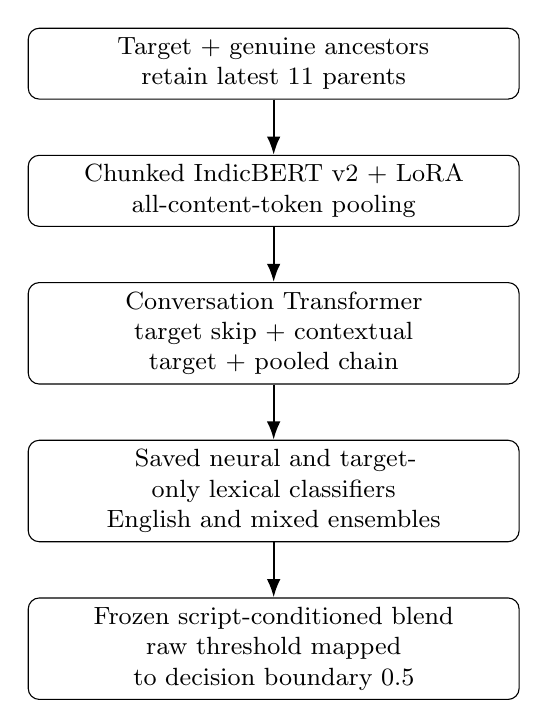
\begin{tikzpicture}[node distance=7mm,box/.style={draw,rounded corners,align=center,font=\small,text width=6.0cm,minimum height=9mm},arr/.style={-{Latex},thick}]
\node[box] (input) {Target + genuine ancestors\\retain latest 11 parents};
\node[box,below=of input] (encoder) {Chunked IndicBERT v2 + LoRA\\all-content-token pooling};
\node[box,below=of encoder] (turn) {Conversation Transformer\\target skip + contextual target + pooled chain};
\node[box,below=of turn] (experts) {Saved neural and target-only lexical classifiers\\English and mixed ensembles};
\node[box,below=of experts] (policy) {Frozen script-conditioned blend\\raw threshold mapped to decision boundary 0.5};
\draw[arr](input)--(encoder);\draw[arr](encoder)--(turn);\draw[arr](turn)--(experts);\draw[arr](experts)--(policy);
\end{tikzpicture}
\caption{Inference components. Lexical classifiers use the target text directly, not the contextual representation. Expert ensembles contain related neural/lexical components; they are not independent model families.}
\end{figure}

\subsection{Adaptation and lexical ensembles}
LoRA targets query and value matrices, with rank 8, scaling parameter 16 and dropout 0.1~\citep{hu2021}. The configured maximum training duration is five epochs with seed 42, batch size 8 and gradient accumulation over four steps. Encoder-adapter and head learning rates are $3\times10^{-5}$ and $3\times10^{-4}$; weight decay is 0.01, gradient clipping is 1.0 and validation patience is three epochs. Training uses class-weighted binary cross-entropy and validation-based epoch/threshold selection. Context dropout is zero in these saved configurations. CUDA training uses mixed precision; the present expert-score export uses FP32.

Lexical candidates use target-only character TF-IDF (3--5 grams) and word TF-IDF (1--2 grams), with logistic classifiers implemented via Scikit-learn~\citep{pedregosa2011}. Original ensemble weights were selected on a quarter-step simplex using the mean of overall and contextual validation AP, followed by an F1-selected validation threshold. The saved English ensemble uses 0.75 character and 0.25 neural weight; the mixed ensemble uses 0.50 character and 0.50 neural weight. Both assign zero weight to the word candidate. A frozen-encoder target-only MLP and frozen hierarchical model exist in the earlier English comparison; the present routing analysis reuses the saved ensembles and mixed neural expert.

\subsection{Conservative adaptive policy}
Let $p_E$, $p_M$ and $p_N$ denote the English ensemble, mixed ensemble and mixed neural scores. A Unicode-based rule inspects the retained target/history and assigns a script bucket $b$. The raw mixture is
\begin{equation}
r_b=w_{bE}p_E+w_{bM}p_M+w_{bN}p_N,\qquad w_{bj}\geq0,\quad\sum_j w_{bj}=1.
\end{equation}
Latin-script input is ambiguous: it may be English or Romanized Indic text. The English contribution is capped at 0.25 for its soft-blend candidate and is excluded from the hard router. Other script buckets use mixed experts; unknown scripts use the existing mixed ensemble. No source identifier is required as an inference input. The selected mixture weights and branch thresholds across detected script groups are listed in Table~\ref{tab:policy}.

For branch threshold $t_b$, a monotone piecewise transform places the decision boundary at 0.5:
\begin{equation}
s_b(r)=\begin{cases}r/(2t_b),&r<t_b,\\
\tfrac12+(r-t_b)/(2(1-t_b)),&r\geq t_b.
\end{cases}
\end{equation}
The implementation handles endpoint thresholds numerically. This is not probability calibration. Although ranking is preserved within each branch, different branch transforms can change ranking across the pooled population.

The original 11,776-row validation population is partitioned into 6,978 fitting and 4,798 selection rows using connected groups and seed 2026. Fitted script routes require at least 100 fitting examples, 15 per class and 15 connected groups; otherwise the fallback applies. Candidate families are the existing mixed ensemble, global mixtures of mixed experts, script hard routing and script soft blending. Their selection objective is the equally weighted mean of source F1 values and contextual-subset F1. Candidates with more than a one-percentage-point source/context F1 regression against the mixed baseline are rejected. Replacement requires more than 0.005 objective gain over the current winner. The selected soft blend has objective 0.76845 versus 0.73088 for the original mixed ensemble on this selection partition.

The base models had already used the original validation set. The partition therefore separates new policy fitting and checking but is not independent of base-model selection. We retain this limitation rather than presenting the procedure as nested cross-validation.

\section{Evaluation Protocol}
We report positive-class F1, precision, recall, AP and confusion counts. Models are evaluated on identical examples within each comparison. Paired percentile intervals resample connected conversation/shared-text groups 1,000 times with seed 2026. The main contextual subset has 2,282 targets in 540 groups; the combined population has 8,882 groups. Intervals are exploratory, unadjusted for multiple comparisons, and do not incorporate training-seed variance or remove prior test-informed development.

Context ablations hold the original routing branch fixed while removing parents. Additional controls reverse ancestor order or replace ancestors with unrelated training-source parents of the same retained length. The target remains unchanged. The controls reuse original labels, so they test sensitivity rather than human-annotated counterfactual accuracy. Reversal is assessed only with at least two ancestors; unrelated replacement reports only eligible examples. Native depth groups are different example populations, not randomized depth interventions.

\section{Results}
% Auto-generated and verified tables for paper_submission/main.tex
% All values derived from saved predictions and verified against reports/adaptive_v1/evaluation.json

\begin{table}[htbp]
\centering\small
\begin{tabular}{lrrrrr}
\toprule
Dataset / Source & Language / Task & Train & Validation & Test & Total \\
\midrule
English CGA & Personal attack (Wiki) & 15,775 (1,221) & 3,480 (285) & 3,577 (274) & 22,832 \\
Telugu safety & Cultural safety prompts & 8,370 (2,516) & 1,800 (534) & 1,787 (569) & 11,957 \\
Tamil code-mixed & Offensiveness (social) & 30,433 (8,472) & 6,496 (1,740) & 6,514 (1,816) & 43,443 \\
\midrule
Combined pool & Multi-task mixture & 54,578 (12,209) & 11,776 (2,559) & 11,878 (2,659) & 78,232 \\
\bottomrule
\end{tabular}
\caption{Cleaned dataset partition counts, with positive (toxic/abusive) counts shown in parentheses. Grouped conversation and shared-text splits prevent cross-split leakage.}\label{tab:data}
\end{table}

\begin{table}[htbp]
\centering\small
\begin{tabular}{lrrrrrr}
\toprule
Model / Training Recipe & Threshold & Overall F1 & Contextual F1 & AP & Precision & Recall \\
\midrule
\multicolumn{7}{l}{\textit{English-Trained Models on English CGA Test ($n=3,577$)}} \\
English char TF-IDF & 0.2239 & 0.7259 & 0.7446 & 0.8049 & 0.7705 & 0.6861 \\
English frozen target-only MLP & 0.7648 & 0.6299 & 0.6267 & 0.6951 & 0.5673 & 0.7080 \\
English frozen contextual Transformer & 0.9457 & 0.6546 & 0.6600 & 0.7322 & 0.6487 & 0.6606 \\
English LoRA contextual Transformer & 0.8228 & 0.7232 & 0.7433 & 0.8194 & 0.7313 & 0.7153 \\
\textbf{English ensemble (75\% char + 25\% LoRA)} & 0.3061 & \textbf{0.7869} & \textbf{0.7981} & \textbf{0.8629} & 0.7435 & 0.8358 \\
\midrule
\multicolumn{7}{l}{\textit{Historical Mixed-Language Models Evaluated on the Identical English Test Set}} \\
Historical mixed TF-IDF & 0.3266 & 0.6035 & 0.6061 & 0.7007 & 0.7611 & 0.5000 \\
Historical mixed LoRA Transformer & 0.5952 & 0.7394 & 0.7612 & 0.8059 & 0.7491 & 0.7299 \\
Historical mixed ensemble & 0.4827 & 0.7459 & 0.7713 & 0.8404 & 0.8505 & 0.6642 \\
\bottomrule
\end{tabular}
\caption{Matched evaluation on identical 3,577 English CGA holdout test targets (274 positives; 2,282 contextual targets with $\ge 1$ ancestors). All models evaluated using their respective validation-selected thresholds.}\label{tab:english_matched}
\end{table}

\begin{table}[htbp]
\centering\small
\begin{tabular}{lrrrrr}
\toprule
Population & English ens. & Mixed neural & Mixed ens. & Adaptive blend & Adaptive AP \\
\midrule
Combined test ($n=11,878$) & 0.1710 & 0.6947 & 0.7284 & 0.7299 & 0.8007 \\
English CGA ($n=3,577$) & \textbf{0.7869} & 0.7394 & 0.7459 & 0.7650 & 0.8563 \\
Telugu safety ($n=1,787$) & 0.0000 & 0.8336 & 0.8419 & \textbf{0.8498} & 0.9200 \\
Tamil code-mixed ($n=6,514$) & 0.0311 & 0.6454 & \textbf{0.6883} & 0.6856 & 0.7371 \\
\bottomrule
\end{tabular}
\caption{Positive-class F1 across expert baselines and the validation-selected adaptive policy, evaluated on the full 11,878 test set. The pure English ensemble collapses on Indic scripts, while adaptive script-conditioned blending balances specialized performance across sources.}\label{tab:main}
\end{table}

\begin{table}[htbp]
\centering\small
\begin{tabular}{lrrrrrr}
\toprule
Source Population & Precision & Recall & F1 & AP & ROC-AUC & Confusion Matrix [TN, FP; FN, TP] \\
\midrule
English CGA ($n=3,577$) & 0.7636 & 0.7664 & 0.7650 & 0.8563 & 0.9789 & [3238, 65; 64, 210] \\
Telugu safety ($n=1,787$) & 0.7789 & 0.9350 & 0.8498 & 0.9200 & 0.9645 & [1067, 151; 37, 532] \\
Tamil code-mixed ($n=6,514$) & 0.6519 & 0.7230 & 0.6856 & 0.7371 & 0.8802 & [3997, 701; 503, 1313] \\
\midrule
Combined test ($n=11,878$) & 0.6915 & 0.7728 & 0.7299 & 0.8007 & 0.9320 & [8302, 917; 604, 2055] \\
\bottomrule
\end{tabular}
\caption{Comprehensive performance breakdown of the selected adaptive policy (\texttt{script\_soft\_blend}) across all source populations on the held-out test split.}\label{tab:adaptive_details}
\end{table}

\begin{table}[htbp]
\centering\small
\begin{tabular}{lrr}
\toprule
Population & $\Delta$F1 (percentage points) & 95\% Group-Bootstrap Interval (pp) \\
\midrule
Combined test ($n=11,878$) & +0.144 & [-0.424, +0.744] \\
English CGA ($n=3,577$) & +1.913 & [-0.956, +5.109] \\
Telugu safety ($n=1,787$) & +0.790 & [-0.513, +2.048] \\
Tamil code-mixed ($n=6,514$) & -0.264 & [-0.842, +0.348] \\
\bottomrule
\end{tabular}
\caption{Paired F1 difference ($\text{Adaptive} - \text{Mixed Ensemble}$) with 1,000 paired connected-group bootstrap resamples (seed 2026). All intervals span zero, indicating that the overall point difference is not statistically significant.}\label{tab:delta}
\end{table}

\begin{table}[htbp]
\centering\small
\begin{tabular}{lrrrrrr}
\toprule
Evaluation Condition & Eligible $n$ & Precision & Recall & F1 & AP & ROC-AUC \\
\midrule
Adaptive full context & 2,282 & 0.7536 & 0.8112 & 0.7813 & 0.8754 & 0.9782 \\
Adaptive removed context & 2,282 & 0.8323 & 0.7092 & 0.7658 & 0.8560 & 0.9739 \\
\midrule
\multicolumn{7}{l}{\textit{Paired difference (Full Context $-$ Removed Context on $n=2,282$ targets):}} \\
\multicolumn{7}{l}{$\Delta\text{F1} = +1.549\text{ pp}$, 95\% CI: $[-1.678, +4.979\text{ pp}]$ (interval crosses zero)} \\
\multicolumn{7}{l}{$\Delta\text{AP} = +1.945\text{ pp}$, 95\% CI: $[+0.616, +3.132\text{ pp}]$ (strictly positive ranking gain)} \\
\midrule
\multicolumn{7}{l}{\textit{Counterfactual Stress Controls (Router held fixed to original input):}} \\
True context (reversal-eligible) & 1,292 & 0.7764 & 0.8389 & 0.8065 & 0.9136 & 0.9845 \\
Reversed ancestor order & 1,292 & 0.7812 & 0.8389 & 0.8091 & 0.9140 & 0.9845 \\
\midrule
True context (donor-eligible) & 2,253 & 0.7512 & 0.8075 & 0.7784 & 0.8728 & 0.9820 \\
Unrelated training-source parents & 2,253 & 0.7525 & 0.8128 & 0.7815 & 0.8727 & 0.9821 \\
\bottomrule
\end{tabular}
\caption{Context ablation and stress control diagnostics on English CGA contextual test targets. Context removal yields an exploratory ranking gain in AP, but the F1 difference interval includes zero, and shuffled/unrelated parent controls exhibit near-identical performance.}\label{tab:context_controls}
\end{table}

\begin{table}[htbp]
\centering\small
\begin{tabular}{rrrrr|lrrrr}
\toprule
\multicolumn{5}{c|}{\textbf{Parent Retention Budget Sweep ($n=3,577$)}} & \multicolumn{5}{c}{\textbf{Observed Natural Ancestry Depth Breakdown}} \\
Budget & Overall F1 & Overall AP & Ctx F1 & Ctx AP & Depth Group & $n$ & Positives & F1 & AP \\
\midrule
0 parents & 0.7763 & 0.8605 & 0.7844 & 0.8794 & 0 ancestors & 9,596 & 2,463 & 0.7259 & 0.7943 \\
1 parent  & 0.7786 & 0.8607 & 0.7876 & 0.8798 & 1 ancestor  & 990 & 47 & 0.7010 & 0.7426 \\
2 parents & 0.7878 & 0.8620 & 0.8000 & 0.8815 & 2 ancestors & 577 & 37 & 0.7952 & 0.9286 \\
3 parents & 0.7943 & 0.8628 & 0.8088 & 0.8823 & 3 ancestors & 355 & 37 & 0.7671 & 0.8995 \\
5 parents & 0.7849 & 0.8629 & 0.7953 & 0.8831 & 4--7 ancestors & 356 & 73 & 0.8267 & 0.9184 \\
11 parents & 0.7869 & 0.8629 & 0.7981 & 0.8832 & 8--11 ancestors & 4 & 2 & 1.0000 & 1.0000 \\
\bottomrule
\end{tabular}
\caption{Left: Fixed parent retention budgets on English CGA test targets. Right: Natural observed ancestry depth breakdown under the adaptive policy. The four deep examples ($8\text{--}11$ ancestors) are insufficient to claim long-history robustness.}\label{tab:budgets}
\end{table}

\begin{table}[htbp]
\centering\small
\begin{tabular}{lrrrrrr}
\toprule
Model / Evaluated System & F1 & AP & Precision & Recall & FP & FN \\
\midrule
Mixed-language LoRA Transformer & 0.6154 & 0.6063 & 0.4848 & 0.8421 & 17 & 3 \\
Mixed-language clean ensemble & \textbf{0.6522} & \textbf{0.7540} & \textbf{0.5556} & 0.7895 & 12 & 4 \\
Pure English ensemble & 0.0000 & 0.4797 & 0.0000 & 0.0000 & 0 & 19 \\
\textbf{Adaptive policy (\texttt{script\_soft\_blend})} & 0.6222 & 0.7515 & 0.5385 & 0.7368 & 12 & 5 \\
\bottomrule
\end{tabular}
\caption{Authored Telugu/Romanized development challenge (51 targets, 19 positives). The English ensemble fails completely due to zero lexical activation, whereas the adaptive policy restores sensitivity without modifying trained weights.}\label{tab:challenge}
\end{table}

\begin{table}[htbp]
\centering\small
\begin{tabular}{lrrrr}
\toprule
Detected Script Group & English Ens. Weight & Mixed Ens. Weight & Mixed Neural Weight & Calibrated Threshold \\
\midrule
\texttt{latin\_ambiguous} & 0.2500 & 0.7500 & 0.0000 & 0.384322 \\
\texttt{mixed\_script}    & 0.0000 & 0.2500 & 0.7500 & 0.484014 \\
\texttt{tamil\_script}    & 0.0000 & 0.7500 & 0.2500 & 0.494095 \\
\texttt{telugu\_script}   & 0.0000 & 1.0000 & 0.0000 & 0.558908 \\
Fallback (Unknown script) & 0.0000 & 1.0000 & 0.0000 & 0.482698 \\
\bottomrule
\end{tabular}
\caption{Frozen validation-selected policy weights and operating thresholds across detected script groups. Script detection serves as a safeguard against lexical failure, not a true language identifier.}\label{tab:policy}
\end{table}

\begin{table}[htbp]
\centering\small
\begin{tabular}{p{4.5cm}p{10.5cm}}
\toprule
Configuration Parameter & Verified Specification / Checkpoint Hash \\
\midrule
Base Neural Encoder & \texttt{ai4bharat/IndicBERTv2-MLM-Sam-TLM} (commit \texttt{bb783337859e3d7957de5ba82766ddea51e8fc3e}) \\
LoRA Target Modules & Attention Query and Value projections ($r=8$, $\alpha=16$, dropout $0.1$) \\
Conversation Transformer & 2 layers, 4 attention heads, $d_{\text{model}}=192$, $d_{\text{ff}}=384$, GELU activation, dropout $0.1$ \\
Maximum Turns Retained & $T \le 12$ turns (up to 11 ancestors plus 1 target reply) \\
Mixed Dataset Artifact & \texttt{data/processed/contextual\_clean\_v1.jsonl} (SHA-256: \texttt{368817cc6203...}) \\
English Dataset Artifact & \texttt{data/processed/english\_cga\_v1.jsonl} (SHA-256: \texttt{df39ad6827c5...}) \\
Execution Environment & Python 3.10.20, PyTorch 2.12.0+cu130, Transformers 5.17.0, PEFT 0.18.1 \\
Hardware & NVIDIA GeForce RTX 4060 Laptop GPU (8,188 MiB VRAM), CUDA 13.0 \\
Software Tests & 95 passed, 1 skipped in 42.69s (\texttt{reports/adaptive\_v1/tests.xml}) \\
Serving Parity & FP32 serving predictor verified with 0 decision flips against trainer predictions \\
\bottomrule
\end{tabular}
\caption{Reproducibility specifications, pinned model configurations, and cryptographic artifact hashes.}\label{tab:reproducibility}
\end{table}


\subsection{Specialization and expert blending}
Table~\ref{tab:english_matched} shows the matched comparison across all investigated models on the identical 3,577 English CGA holdout test set. The English ensemble (75\% character TF-IDF and 25\% LoRA Transformer) achieves F1 of 0.7869 and AP of 0.8629, outperforming both standalone English components and the historical mixed-language models. However, as shown in Table~\ref{tab:main}, the English specialist fails to transfer to Indic sources (F1 of 0 on Telugu safety and 0.0311 on Tamil code-mixed inputs). 

Table~\ref{tab:adaptive_details} provides the complete performance breakdown of the selected adaptive policy (\texttt{script\_soft\_blend}) across all evaluation splits. On the combined test population ($n=11,878$), adaptive F1 is 0.7299 versus 0.7284 for the mixed ensemble. As reported in Table~\ref{tab:delta}, the paired difference is only +0.144 percentage points, with a 95\% interval of $[-0.424,+0.744]$ points. AP decreases from 0.8041 to 0.8007. The adaptive confusion matrix is $\left[\begin{smallmatrix}8302&917\\604&2055\end{smallmatrix}\right]$ versus $\left[\begin{smallmatrix}8324&895\\623&2036\end{smallmatrix}\right]$ for the mixed ensemble: 19 additional true positives come with 22 additional false positives. Source-level F1 differences against the mixed ensemble also have intervals containing zero. These results do not establish that adaptive blending improves overall performance.

\subsection{Does parent context help?}
Table~\ref{tab:context_controls} presents the full context ablation and counterfactual stress control diagnostics on the 2,282 contextual English targets. Adaptive full-context F1 is 0.7813 versus 0.7658 without parents. The +1.549-point difference has interval $[-1.678,+4.979]$, so the F1 benefit remains uncertain. AP increases from 0.8560 to 0.8754: +1.945 points with interval $[+0.616,+3.132]$. This supports an exploratory ranking advantage under the measured protocol, not a broad claim of better toxicity decisions.

The controls in Table~\ref{tab:context_controls} further constrain interpretation. On 1,292 reversal-eligible targets, reversed context obtains F1 0.8091 and AP 0.9140, versus 0.8065 and 0.9136 with original order. On 2,253 unrelated-context-eligible targets, unrelated context obtains F1 0.7815 and AP 0.8727, versus genuine-context F1 0.7784 and AP 0.8728 on that same subset. Thus the measured controls show little separation from genuine ancestry. They do not demonstrate that semantic use of correct parents causes the removal-ablation ranking gain.

Table~\ref{tab:budgets} details the parent retention budget sweep ($0 \to 11$ parents) on English CGA test targets, juxtaposed with the natural observed ancestry depth breakdown under the adaptive policy. Depth groups include 990 targets with one ancestor, 577 with two, 355 with three, 356 with four to seven, and only four with eight to eleven. There are no main-test examples with twelve or more ancestors. The perfect result on four deep examples does not establish long-history robustness.

\subsection{Authored Telugu/Romanized challenge}
Table~\ref{tab:challenge} summarizes the evaluation on the 51 authored Telugu/Romanized development challenge targets. The English ensemble predicts every challenge example negative, missing all 19 positives. Adaptive F1 recovers to 0.6222, but remains below the mixed ensemble's 0.6522. Adaptive makes five false negatives and twelve false positives; the mixed ensemble makes four and twelve. Adaptive minus mixed F1 has interval $[-10.970,0.000]$ percentage points on this small development set. We retain the frozen policy for reporting instead of using challenge labels to select a replacement. No language-wide accuracy or reliable Telugu-context conclusion follows from this set.

\section{Reproducibility, Limitations and Ethics}
Table~\ref{tab:reproducibility} provides the complete reproducibility specification, pinned base encoder commits, artifact SHA-256 hashes, and verified software execution environment. The mixed prepared-data SHA-256 is recorded in the accompanying evidence audit; the English subset and validation-score identities are also frozen in project artifacts. A review of the local return archive verified all 64 manifest entries and independently recomputed key metrics and policy-to-prediction parity, totaling 221 successful checks. Returned software evidence records 95 passing tests and one skipped optional legacy transliteration test. The returned localhost health, benchmark and prediction checks passed for the CPU adaptive demo. These software checks are not model-quality guarantees.

The recorded environment is Python 3.10.20, PyTorch 2.12.0+cu130 and an RTX 4060 Laptop GPU with approximately 8 GB VRAM for scoring. We omit speed claims because narrative notes and score-artifact elapsed times disagree. No additional training or neural inference was performed to produce this manuscript's audit.

Limitations include source/domain and label mismatch, isolated Indic training inputs, a small authored challenge, single configured training seeds, prior validation/test reuse, possible semantic duplicates, and sparse deep-history groups. Script-based routing is not language identification. Threshold-normalized scores are uncalibrated, attention is not a causal explanation, and acceptance of an input does not demonstrate accuracy on its language or depth. Automated predictions should support human review rather than be interpreted as definitive judgments about people. Data redistribution requires checking original and derived-source permissions; public availability alone is insufficient evidence of rights.

\section{Conclusion}
The project provides a working, auditable integration of target-aware hierarchical encoding and lexical/neural expert combinations. The English specialist performs well within its source but transfers poorly to Indic sources. Conservative blending reduces that transfer failure yet does not show a clear overall F1 advantage over the mixed ensemble and regresses on the authored Telugu challenge. Parent removal suggests an exploratory AP advantage, while F1 uncertainty and weak control separation prevent a strong semantic-context claim. Fresh independently annotated conversational data and locked evaluation would be needed for stronger cross-language and context-benefit conclusions.

\bibliographystyle{plainnat}
\bibliography{references}
\end{document}
